\section{Authentication}

As defined by the RFC-4949 \cite{shirey2007internet}, authentication is "The process of verifying a claim that a system entity or system resource has a certain attribute value."
This is a generic definition, and it most frequently applies to the verification of user identity (e.g at login), however assertions can be made and verified about any subject or object.
\\
\\
The authentication process consists of two steps.
\paragraph{Identification} Presenting an identifier to the authentication system, that establishes the entity being authenticated.
In common user authentication systems this is a username or an email verified in the registration process. The identifier needs to be unique for the entity it identifies.

\paragraph{Verification} Presenting or generating authentication information that can be used to verify the claim.
Commonly used authentication information are passwords, one-time tokens, digital signatures.

\subsection{The NITS Model for Digital Identity}

Digital Identity Guidelines \cite{grassi2017} published by the National Institute of Standards and Technology (NIST) describes a simple digital identity model, that provides a generic authentication framework.

The process has distinct steps of \textit{Enrolment and Identity Proofing} and \textit{Authentication}.

\paragraph{Enrolment and Identity Proofing}

The enrolment describes a process where an \textit{applicant} becomes a \textit{subscriber} after being successfully \textit{proofed} by a \textit{CSP}.
The subscriber is issued a \textit{credential} and one or more \textit{authenticators}.

A common application of this process is user registration on websites.

\paragraph{Authentication}

The claimant begins authentication with the verifier by sharing the credential and the authenticators. The verifier validates binding between the credential and authenticators with the CSP.
An authenticated connection is established between the subscriber and the RP after and assertion is provided by the CSP or the verifier to the RP.

A common application of this is user \textit{login} on websites.


\begin{figure*}[h!]
	\centering
	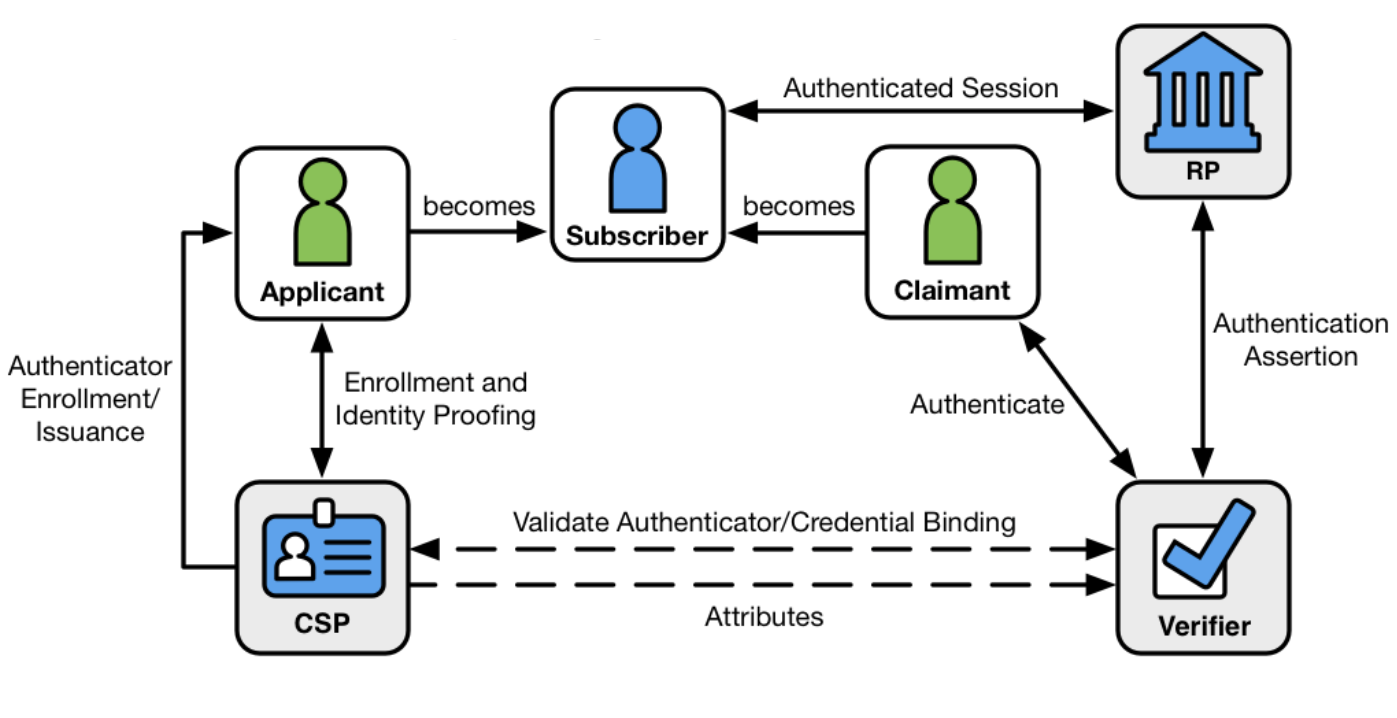
\includegraphics[width=13cm]{images/NIST_digital_identity_model}
	\caption{NITS Digital Identity Model}
	\label{fig:NIST-digital-identity-model}
\end{figure*}

\paragraph{Note on delegation of roles}
In the digital identity model \ref{fig:NIST-digital-identity-model} roles of CSP, verifier and RP are distinct in their responsibility. 
In practice however all these roles can be performed by a single party (e.g any website with native registration and login).

In OAuth2's \cite{hardt2012oauth} authentication layer, the resource owner has the roles of applicant, claimant and subscriber. The authorisation server has the roles of CSP and verifier. The OAuth2 client has the role of the RP.

\subsection{Authentication Factors}

As described in \cite{council2005authentication} authentication systems can rely on three distinct "factors".

\begin{itemize}
	\item \textbf{Knowledge factors} - Something the user \textbf{knows} (e.g, password, security question, PIN)
	\item \textbf{Ownership factors} - Something the user \textbf{owns} (e.g, ID card, security tokens, mobile devices)
	\item \textbf{Inherence factors} - Something the user \textbf{is} or \textbf{does} (e.g, static biometrics - fingerprints, retina, face. dynamic biometrics - voice patterns, typing rhythm)
\end{itemize}

\paragraph{Strong authentication} as defined by government and financial institutions is, an authentication procedure based two or more authentication factors. Authentication using two or more factors is also referred to as \textit{multi-factor authentication}.

\subsection{Password based Authentication}

Passwords are one of the oldest forms of authentication, dating back to ancient times when it was used in the Roman military. It was first used in computers at MIT in the mid-60s \cite{mcmillan2012password}.

% High level arch
Password based authentication is a simple authentication model, based on a shared secret between a user and a system. The secret (password) is used in a combination with a user ID. Most common passwords are a set of characters and are memorised by the user.

Using NIST Digital Identity Guidelines terminology \cite{grassi2017}, the password and the user ID are issued as a credential and an authenticator to the applicant after successful enrolment by the CSP.
A claimant then uses the credentials to authenticate with the verifier, as to establish an authenticated session with the RP.


% Security considerations
\subsubsection{Security}

The simplicity of password-based authentication is also its downside, and the IT community has actively been working to move away from password based authentication and its downsides.
While there are many general attack vectors in any authentication system such as network conditions (man-in-the-middle) and the integrity of the system (viruses, key-loggers). The biggest risk specific to a password-based authentication system is choosing, handling and storing the passwords.

Passwords need to be memorised by the user, which creates an incentive for users to pick passwords that are shorter in length and contain less variance \cite{conklin2004password}.

Ways in which adversaries can attack a PBS can be generally categories based on attackers access to "authenticator data", NIST \cite{grassi2017} classifies \textit{online} and \textit{offline} attacks as.

\paragraph{Online attack} An attack where the attacker assumes the role of the claimant with a genuine verifier.
A common type of attack is a \textit{guessing attack}, where and adversary repeatedly attempts to authenticate with the verifier by guessing possible passwords, this makes the attack very noisy and easy to detect and mitigate.


\paragraph{Offline attack} An attack where an attacker is able to analyse data in a system he controls. Data was obtained by the attacker by either theft of file, eavesdropping an authentication protocol or a system penetration.

Protecting against an offline attack means making it very expensive for an attacker to guess the password or "crack the password".
What influences the cost of guessing a password is the expected password entropy and the time to guess a single password.

\subparagraph{Password storage}
An important defence against offline attack are the methods with which passwords are stored and verified.
Trivially passwords stored in plaintext or hashed passwords are easy for an attacker to exploit efficiently with methods like pre-computed hash and rainbow tables. 

Modern password based security relies on methods of key-derivation that make password cracking both time-consuming and memory-hard \cite{percival2016scrypt, biryukov2016argon2, boneh2016balloon} and using \textit{salt} \cite{hornby2016salted} to make pre-computation attacks infeasible.
Key-derivation functions transform the plain text passwords into password hashes for storage.
When the system wants to verify a password it repeats the process of key-derivation and compares the output hash with the one in storage.

\subparagraph{Password strength}
\textit{The strength} of a password directly relates to its entropy. The overall cost password cracking can be reduced by orders of magnitude by a week password, because the attacker has a smaller pool of passwords to try.
Have I Been Pwned \cite{hunt2021have} catalogs 613,584,248 passwords recovered from data breaches, while CrackStation \cite{hornby2019password} lists a collection of 1,493,677,782 words used for password cracking. Any password cracking software will exhaust the list in relatively short time compared to a brute-forcing technique.








